\documentclass{beamer}

\usepackage[utf8]{inputenc}
\usepackage[frenchb]{babel}
\usepackage{verbatim}
\usepackage{graphicx}
\usepackage{color}
\usepackage{hyperref}
\usepackage{verbatim}
\usepackage{url}
\usepackage{auto-pst-pdf}
\usepackage{pst-plot}
\usepackage{moreverb}
\usepackage{fancyvrb}
\usepackage{minted}
\usepackage{algpseudocode}
\usepackage{natbib}
\usepackage{eulervm}

\hypersetup{colorlinks=true, linkcolor=black, urlcolor=blue}
\usetheme{boxes}
\beamertemplatenavigationsymbolsempty
\setbeamertemplate{sections/subsections in toc}[circle]
\setbeamertemplate{footline}[frame number]
\setbeamertemplate{itemize items}[circle]
\setbeamertemplate{itemize subitem}[square]

\title{{\bf Understanding Random Forests}\\
From Theory to Practice}
\author{Gilles Louppe}
\institute{Université de Liège, Belgium}
\date{October 9, 2014}

\newcommand{\todo}[1]{\textcolor{red}{[TODO] #1}}

\definecolor{lightgreen}{rgb}{0.0,0.8,0.0}
\definecolor{lightblue}{rgb}{0.3,0.8,1.0}
\definecolor{lightred}{rgb}{0.874,0.180,0.105}
\definecolor{gray}{rgb}{0.4,0.4,0.4}
\definecolor{lightgray}{rgb}{0.8,0.8,0.8}
\definecolor{shadecolor}{rgb}{0.9,0.9,0.9}
\newrgbcolor{mygreen}{.00 .5 .00}
\newrgbcolor{myyellow}{.6 .6 .00}

\DeclareMathOperator*{\argmax}{arg\,max}


\newrgbcolor{mygreen}{.00 .5 .00}
\newcommand{\X}[1]{\textcolor{blue}{#1}}
\newcommand{\y}[1]{\textcolor{red}{#1}}
\newcommand{\model}[1]{\textcolor{mygreen}{#1}}
\newcommand{\loss}[1]{\textcolor{lightblue}{#1}}

\begin{document}

% Title page ==================================================================

\begin{frame}
\titlepage
\end{frame}


% Motivation ==================================================================

\begin{frame}
  \frametitle{Outline}
  \tableofcontents
\end{frame}

\section{Motivation}
% Mention what is not included in this talk

\begin{frame}{Motivation}

\begin{figure}
\vspace{-0.5cm}
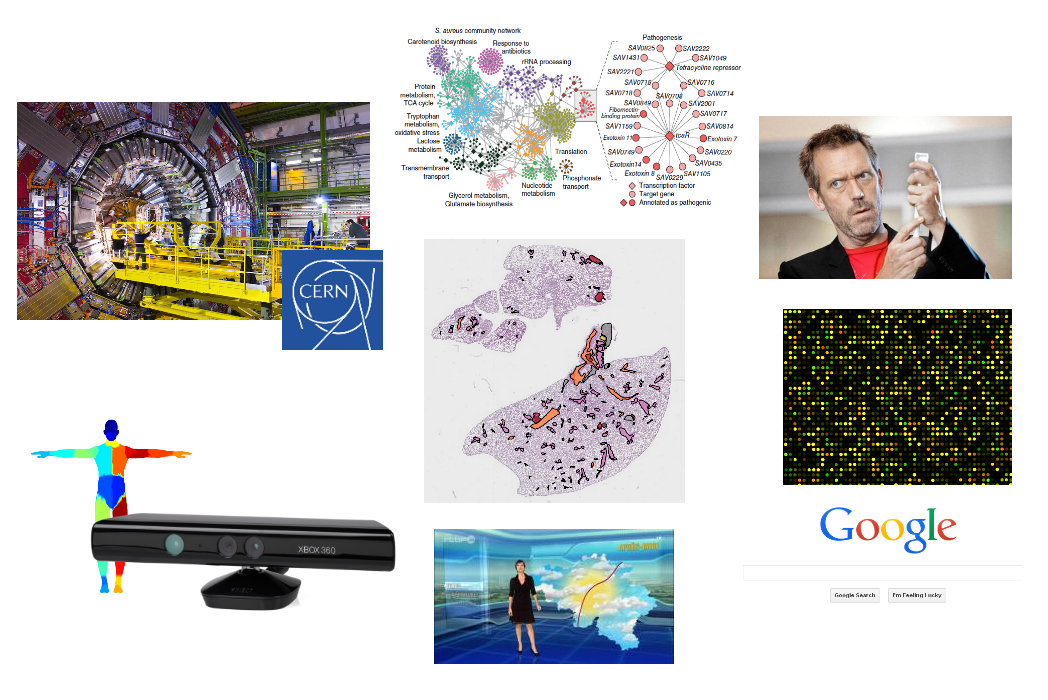
\includegraphics[scale=0.4]{./figures/motivation.png}
\end{figure}

% concrete example => predict output from a set of measurements
% use a continuous example all throughout the slides
% quality of wine from physicochemical properties
\end{frame}

\begin{frame}{Objective}

\begin{center}
From a set of {\bf \X{measurements}},

\vspace{1cm}
learn a {\bf \model{model}}
\vspace{1cm}

to predict and understand {\bf \y{a phenomenon}}.
\end{center}

\end{frame}

\begin{frame}{Running example}

\begin{columns}
\begin{column}{0.5\textwidth}

\begin{center}
From {\bf \X{physicochemical properties}} (alcohol, acidity, sulphates, ...),

\vspace{1cm}
learn a {\bf \model{model}}
\vspace{1cm}

to predict {\bf \y{wine taste preferences}} (from 0 to 10).

\end{center}

\end{column}
\begin{column}{0.5\textwidth}
  \begin{figure}
  \vspace{-0.5cm}
  
\includegraphics[scale=0.6]{./figures/wine.jpg}
  \end{figure}
\end{column}
\end{columns}

\vspace{1cm}

{\footnotesize
P. Cortez, A. Cerdeira, F. Almeida, T. Matos and J. Reis,
{\it Modeling wine preferences by data mining from physicochemical properties},
2009.}

\end{frame}


% Supervised learning =========================================================

\AtBeginSection[]
{
\begin{frame}
  \frametitle{Outline}
  \tableofcontents[currentsection]
  % Die Option [pausesections]
\end{frame}
}

\section{Growing decision trees}

\begin{frame}{Supervised learning}

\begin{itemize}
\item The \X{inputs} are random variables \X{$X = X_1$, ..., $X_p$};
\item The \y{output} is a random variable \y{$Y$}.
\end{itemize}

\begin{itemize}
\item Data comes as a finite learning set $${\cal L} = \{(\X{\mathbf{x}_i}, \y{y_i}) | i = 0, \dots, N-1 \},$$
where \X{$\mathbf{x}_i \in {\cal X} = {\cal X}_1 \times ... \times {\cal X}_p$} and \y{$y_i \in {\cal Y}$}
are randomly drawn from $P_{\X{X},\y{Y}}$.\\
\vspace{0.3cm}
E.g., $(\X{\mathbf{x}_i}, \y{y_i}) = ((\X{\text{color}=\text{red}}, \X{\text{alcohol}=12}, ...), \y{\text{score}=6})$
\end{itemize}

\begin{itemize}
\item The goal is to find a model $\model{\varphi_{\cal L}}: \X{{\cal X}} \mapsto \y{{\cal Y}}$ minimizing
$$
Err(\model{\varphi_{\cal L}}) = \mathbb{E}_{\X{X}, \y{Y}}\{ L(\y{Y}, \model{\varphi_{\cal L}}(\X{X})) \}.
$$
\end{itemize}

\end{frame}

\begin{frame}{Performance evaluation}

\begin{itemize}

\item {\it Classification} (e.g. ${\cal Y} = \{ \text{yes}, \text{no} \}$):
  $$L(Y, \varphi_{\cal L}(X)) = 1(Y \neq \varphi_{\cal L}(X))$$
  {\it \footnotesize (Number of times the predictions are wrong.)}

\vspace{1cm}

\item {\it Regression} (e.g. ${\cal Y} = \mathbb{R}$):
  $$L(Y, \varphi_{\cal L}(X)) = (Y - \varphi_{\cal L}(X))^2$$
  {\it \footnotesize (Large errors are more penalized.)}

\end{itemize}

\end{frame}


% Decision trees ==============================================================

\begin{frame}{Divide and conquer}
\begin{figure}
\only<1>{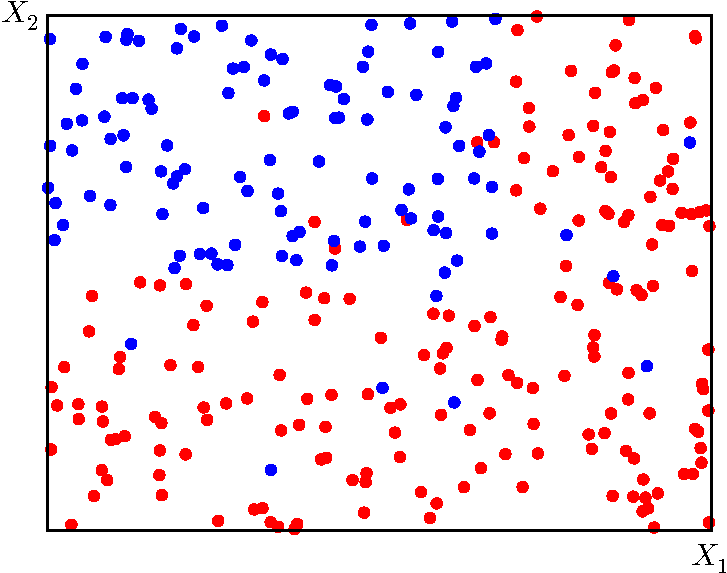
\includegraphics[scale=0.75]{./figures/tree-partition-c.pdf}}
\only<2>{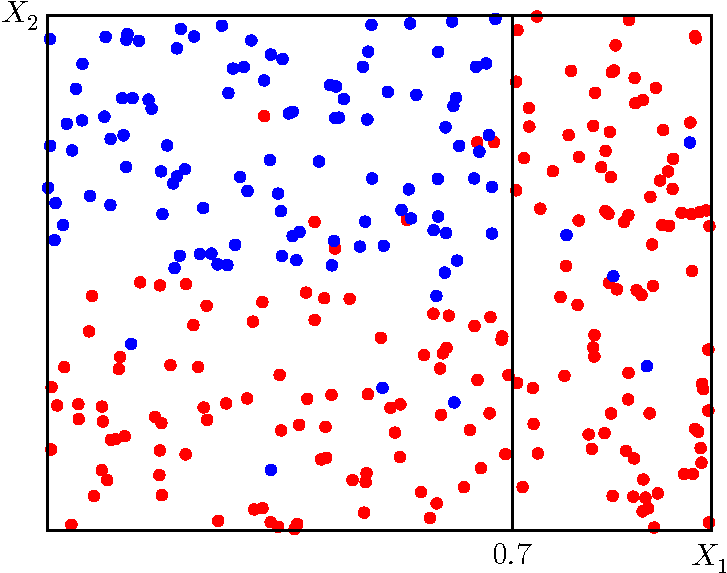
\includegraphics[scale=0.75]{./figures/tree-partition-b.pdf}}
\only<3>{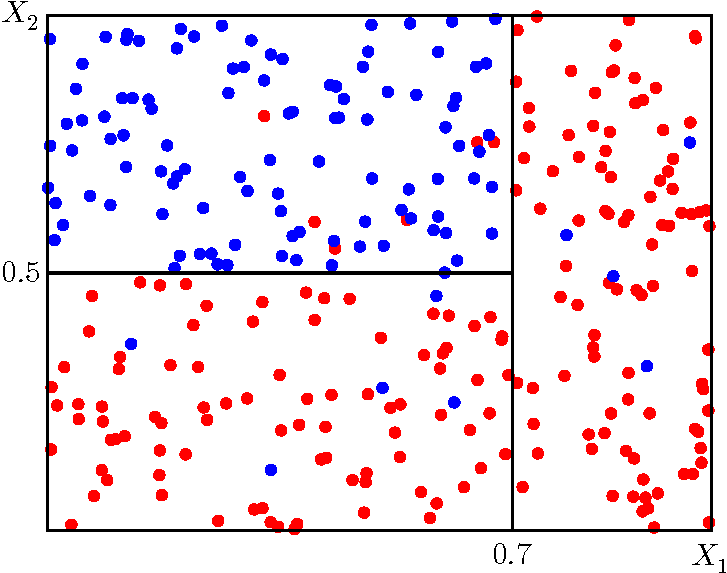
\includegraphics[scale=0.75]{./figures/tree-partition-a.pdf}}
\end{figure}
\end{frame}

\begin{frame}{Decision trees}
\begin{figure}
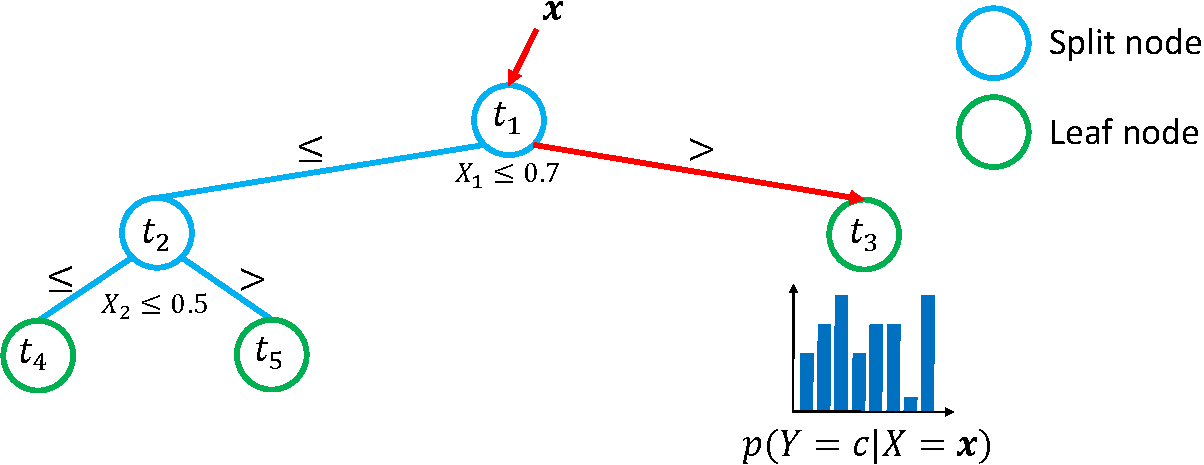
\includegraphics[scale=0.5]{./figures/tree-simple.pdf}
\end{figure}

$t \in \varphi$: nodes of the tree $\varphi$\\
$X_t$: split variable at $t$ \\
$v_t \in \mathbb{R}$: split threshold at $t$\\
$\varphi(\mathbf{x}) = \argmax_{c \in {\cal Y}} p(Y = c | X = \mathbf{x})$
\end{frame}

\begin{frame}{Back to our example}
\begin{figure}
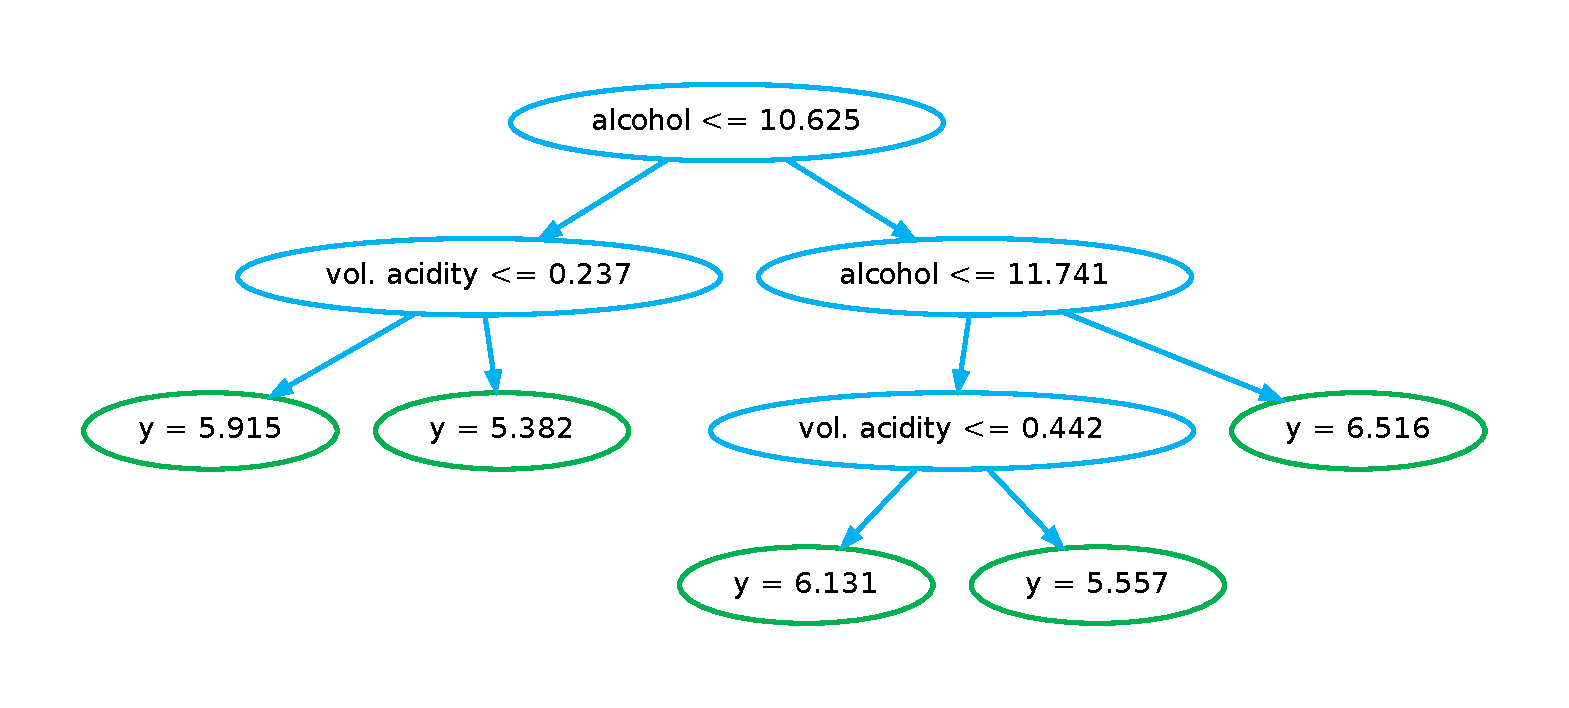
\includegraphics[scale=0.4]{./figures/tree-wine.pdf}
\end{figure}
\end{frame}

% Bias-variance ===============================================================

\begin{frame}{Bias-variance decomposition}

\begin{columns}
\begin{column}{0.65\textwidth}

{\bf Theorem.} For the squared error loss, the bias-variance decomposition of the expected
generalization error at $X=\mathbf{x}$ is
\begin{equation*}
\mathbb{E}_{\cal L} \{ Err(\varphi_{\cal L}(\mathbf{x})) \} = \text{noise}(\mathbf{x}) + \text{bias}^2(\mathbf{x}) + \text{var}(\mathbf{x})
\end{equation*}
where
\begin{align*}
\text{noise}(\mathbf{x}) &= Err(\varphi_B(\mathbf{x})), \\
\text{bias}^2(\mathbf{x}) &= (\varphi_B(\mathbf{x}) - \mathbb{E}_{\cal L} \{ \varphi_{\cal L}(\mathbf{x}) \} )^2, \\
\text{var}(\mathbf{x}) &= \mathbb{E}_{\cal L} \{ (\mathbb{E}_{\cal L} \{ \varphi_{\cal L}(\mathbf{x}) \} - \varphi_{\cal L}(\mathbf{x}))^2 \}.
\end{align*}

\end{column}
\begin{column}{0.35\textwidth}

\begin{figure}
\vspace{-1cm}
\hspace*{-0.4cm}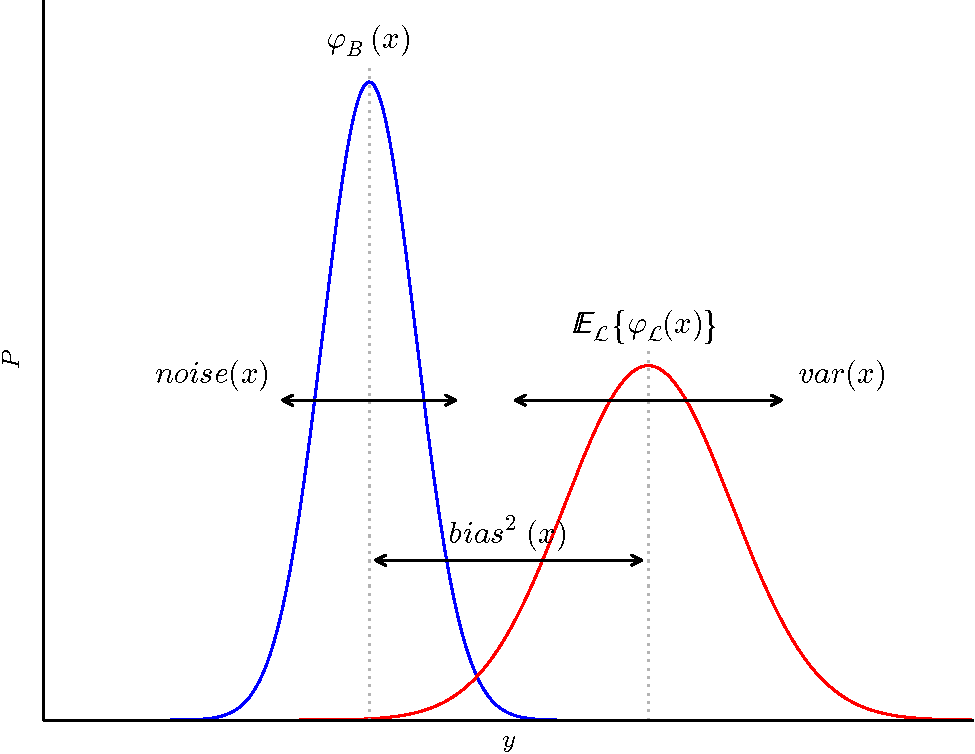
\includegraphics[scale=0.3]{./figures/bias-variance.pdf}\\
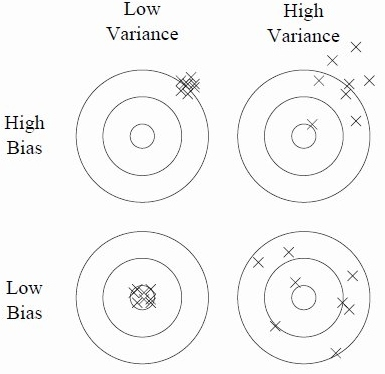
\includegraphics[scale=0.4]{./figures/bias-variance-darts.jpg}
\end{figure}

\end{column}
\end{columns}

% Condorcet Jurys theorem => make people vote on wine quality
% Answer why making several trees help reduce the error
% even if they are built at random!
\end{frame}

\begin{frame}{Diagnosing the generalization error of a decision tree}

\begin{itemize}
\item Residual error: Lowest achievable error, independent of $\varphi_{\cal L}$.
\item Bias: Decision trees usually have {\color{blue} low bias}.
\item Variance: They often suffer from {\color{red} high variance}.
\end{itemize}

\begin{itemize}
\item Solution: {\it Combine the predictions of several randomized trees into a single model.}
\end{itemize}

\end{frame}


% Forests =====================================================================

\begin{frame}{Random forests}
\begin{figure}
    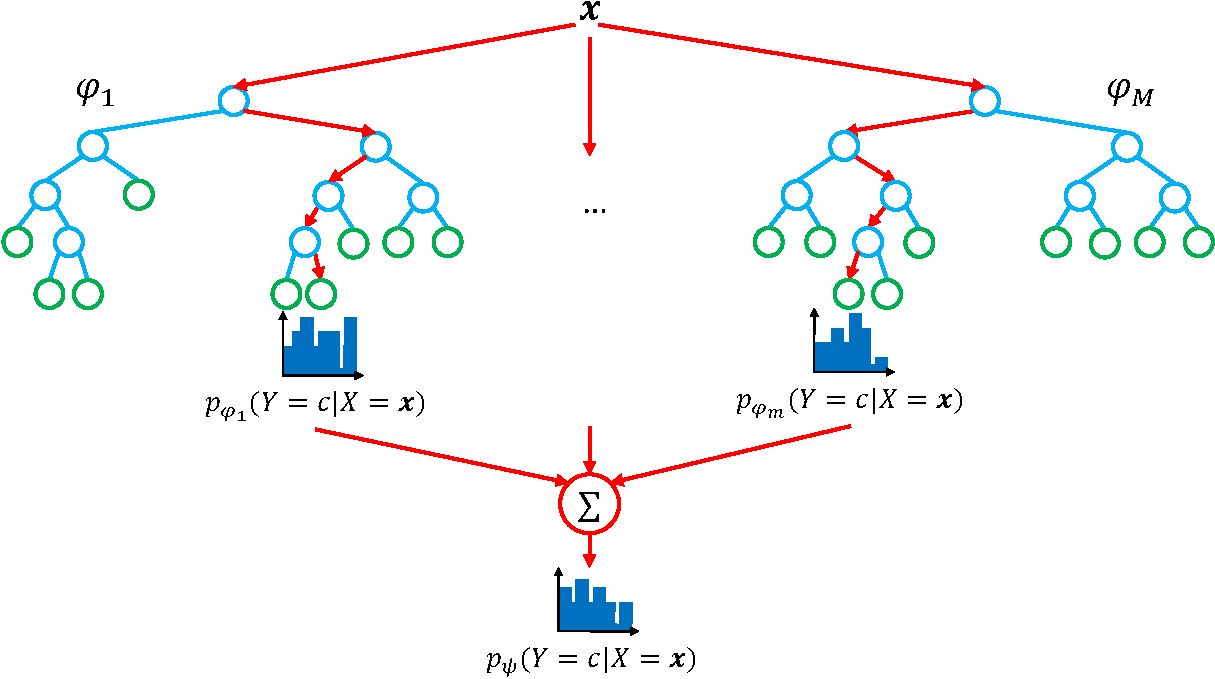
\includegraphics[scale=0.5]{./figures/forest.pdf}
\end{figure}

Ensemble of $M$ randomized decision trees $\varphi_m$\\
$\psi(\mathbf{x}) = \argmax_{c \in {\cal Y}} \frac{1}{M} \sum_{m=1}^M p_{\varphi_m}(Y = c | X = \mathbf{x})$
\end{frame}

\begin{frame}{Condorcet's jury theorem}

\begin{columns}
\begin{column}{0.65\textwidth}
Let consider a group of $M$ voters.

\vspace{1cm}

If each voter has an independent  probability $p > \tfrac{1}{2}$ of voting for
the correct decision, then adding more voters increases the probability of the
majority decision to be correct.

\vspace{1cm}

When $M \to \infty$, the probability that the
decision taken by the group is correct approaches $1$.

\end{column}

\begin{column}{0.35\textwidth}
\begin{figure}
    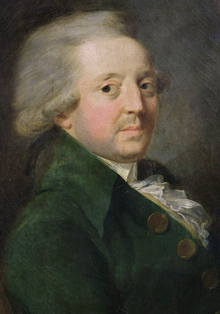
\includegraphics[scale=1.0]{./figures/condorcet.png}
\end{figure}
\end{column}
\end{columns}

\end{frame}


\begin{frame}{Bias-variance decomposition (cont.)}

{\bf Theorem.}
For the squared error loss, the bias-variance decomposition of the expected
generalization error $\mathbb{E}_{\cal L} \{ Err( \psi_{{\cal L},\theta_1,\dots,\theta_M}(\mathbf{x}))
\}$ at $X=\mathbf{x}$ of an ensemble of $M$ randomized models $\varphi_{{\cal L},\theta_m}$ is
\begin{equation*}
\mathbb{E}_{\cal L} \{ Err(\psi_{{\cal L},\theta_1,\dots,\theta_M}(\mathbf{x})) \} = \text{noise}(\mathbf{x}) + \text{bias}^2(\mathbf{x}) + \text{var}(\mathbf{x}),
\end{equation*}
where
\begin{align*}
\text{noise}(\mathbf{x}) &= Err(\varphi_B(\mathbf{x})), \\
\text{bias}^2(\mathbf{x}) &= (\varphi_B(\mathbf{x}) - \mathbb{E}_{{\cal L},\theta} \{ \varphi_{{\cal L},\theta}(\mathbf{x}) \} )^2, \\
\text{var}(\mathbf{x}) &= \rho(\mathbf{x}) \sigma^2_{{\cal L},\theta}(\mathbf{x}) + \frac{1 - \rho(\mathbf{x})}{M} \sigma^2_{{\cal L},\theta}(\mathbf{x}).
\end{align*}

and where $\rho(\mathbf{x})$ is the Pearson correlation coefficient between the predictions of two randomized trees built on the same learning set.

\end{frame}

\begin{frame}{Interpretation of $\rho(\mathbf{x})$}

{\bf Theorem.} $\rho(\mathbf{x}) = \frac{\mathbb{V}_{\cal L} \{ \mathbb{E}_{\theta|{\cal L}} \{ \varphi_{{\cal L},\theta}(\mathbf{x}) \} \}}{\mathbb{V}_{\cal L} \{ \mathbb{E}_{\theta|{\cal L}} \{ \varphi_{{\cal L},\theta}(\mathbf{x}) \} \} + \mathbb{E}_{\cal L} \{ \mathbb{V}_{\theta|{\cal L}} \{ \varphi_{{\cal L},\theta}(\mathbf{x}) \} \}}$

\vspace{1cm}

In other words, it is the ratio between
\begin{itemize}
\item the variance due to the learning set and
\item the total variance, accounting for random effects due to both the learning set and the random perburbations.
\end{itemize}

\begin{itemize}
\item $\rho(\mathbf{x}) \to 1$ when variance is mostly due to the learning set;
\item $\rho(\mathbf{x}) \to 0$ when variance is mostly due to the random perturbations.
\end{itemize}

\end{frame}

\begin{frame}{Diagnosing the generalization error of random forests}

\begin{itemize}
\item Residual error: Lowest achievable error, independent of $\psi_{\cal L}$.
\item Bias: {\color{blue} Identical} to the bias of a single randomized tree.
\item Variance: As $M \to \infty$, {\color{red} $\text{var}(\mathbf{x}) \to \rho(\mathbf{x}) \sigma^2_{{\cal L},\theta}(\mathbf{x})$}
  \begin{itemize}
    \item The stronger the randomization, $\rho(\mathbf{x}) \to 0$, $\text{var}(\mathbf{x}) \to 0$.
    \item The weaker the randomization, $\rho(\mathbf{x}) \to 1$, $\text{var}(\mathbf{x}) \to \sigma^2_{{\cal L},\theta}(\mathbf{x})$
  \end{itemize}
\end{itemize}

\vspace{1cm}

{\bf Bias-variance trade-off.} Randomization increases bias but makes it
possible to reduce the variance of the corresponding ensemble model. The crux
of the problem is to {\color{red} find the right trade-off}.

\end{frame}

\begin{frame}{Back to our example}

\begin{table}
    \centering
    \begin{tabular}{| l c c |}
    \hline
        \textit{Method} & \textit{Trees} & \textit{MSE}  \\
    \hline
    \hline
    CART & 1 & 1.055 \\
    Random Forest & 50 & 0.517 \\
    Extra-Trees & 50 & 0.507 \\
    \hline
    \end{tabular}
\end{table}

\vspace{0.5cm}

\begin{center}
Combining several randomized trees works better!
\end{center}

\end{frame}


% Bias-variance ===============================================================

\section{Interpreting random forests}


\begin{frame}{Variable importances}
% Show them => How to interpret them?
% MDA + MDI
\end{frame}

\begin{frame}{Mean decrease of impurity}
% Motivation
\end{frame}

\begin{frame}{Working assumptions}
\end{frame}

\begin{frame}{Result 1: Three-level decomposition}
\end{frame}

\begin{frame}{Result 2: Irrelevant variables}
\end{frame}

\begin{frame}{Non-totally randomized trees}
\end{frame}

\begin{frame}{Further insights}
% Source of bias
\end{frame}


% Computational performance ===================================================

\section{Computational performance}

\begin{frame}{Complexity}
\end{frame}

\begin{frame}{Implementation}
\end{frame}

\begin{frame}{Random patches}
\end{frame}


% Conclusions =================================================================

\section{Conclusions}

\begin{frame}{Conclusions}
\end{frame}

\end{document}
